
%%%%%%%%%%%%%%%%%%%%%%%%%%%%%%%%%%%%%%%%%%%%%%%%%%%%%%%%%%%%%%%%%% Preamable %%%%%%%%%%%%%%%%%%%%%%%%%%%%%%%%%%%%%%%%%%%%%%%%%%%%%%%%%%%%%%%%%%

% Document Class
\documentclass[pdftex,12pt,a4paper]{article}

% Loading Packages
\usepackage{verbatim}					% Reimplements the verbatim environment, which reproduces text as text - i.e. instead of running it as a LaTeX command
\usepackage{epigraph}					% For epigraphs
\usepackage[nottoc,numbib]{tocbibind}	% Required to list the bibliograpy in the table of contents
\usepackage{gensymb}					% Provides generic commands \degree, \celsius, \perthousand, \micro & \ohm, which work in both text and maths mode
\usepackage{fixltx2e}					% Package containing subscripting & superscripting functions: \textsubscript{text to be subscripted} & \textsuperscript{text to be superscripted}
\usepackage{amssymb, amsmath}			% Import math packages so mathematical symbols are available for equations
\usepackage{pdflscape}					% Produce landscape pages in a (mainly) portrait document. \begin{landscape} & \end{landscape} to change the margins and rotate the page contents, but not the page number.
\usepackage[left=2cm,right=2cm,top=2cm,bottom=2cm]{geometry}	% Geometry package is used for setting margins
\usepackage{siunitx}					% A package for working with SI units
\usepackage[usenames, dvipsnames]{color}	% Text-colouring package
\usepackage[english]{babel}				% 'Multilingual support for Plain TEX or LATEX'
\usepackage{blindtext}					% Useful for creating dummy text to act as an example or a placeholder
\usepackage{amsfonts}					% 'An extended set of fonts for use in mathematics'
\usepackage{upgreek}					% 'A package to provide the upright Greek letters from the Euler or Adobe Symbol fonts as additional math symbols'
\usepackage{graphicx}			% 'Builds upon the graphics package, providing a keyvalue interface for optional arguments to the \includegraphics command'
\usepackage[font=footnotesize,labelfont=bf]{caption}	% 'Provides many ways to customise the captions in floating environments like figure and table'
\usepackage[font=footnotesize,labelfont=bf]{subcaption}	% 'Provides a means of using facilities analagous to those of the caption pack­age, when writing captions for subfigures and the like'
\usepackage{lmodern}					% 'Sets up text fonts so that the Latin Modern family is used'
\usepackage{fancyhdr}					% 'Provides extensive facilities, both for constructing headers and footers, and for controlling their use'
\usepackage{enumitem}					% 'Provides user control over the layout of the three basic list environments: enumerate, itemize and description'
\usepackage{eurosym}					% 'European currency symbol for the Euro implemented in METAFONT'
\usepackage{dcolumn}					% Align table columns on decimal point
\usepackage{bm}							% Bold math
\usepackage{booktabs}					% 'Enhances the quality of tables in LATEX, providing extra commands as well as behind-the-scenes optimisation'
\usepackage{multirow}					% 'Create tabular cells spanning multiple rows'
\usepackage{framed}						% 'Framed or shaded regions that can break across pages'
\usepackage{url}						% 'Verbatim with URL-sensitive line breaks'
\usepackage{pgfgantt}					% 'Draw Gantt charts with TikZ'
\usepackage[super]{nth}					% 'Generate English ordinal numbers'
\usepackage{array}						% 'Extending the array and tabular environments'
\usepackage{calc}  						% 'Simple arithmetic in LATEX commands'
\usepackage{cite}						% 'Improved citation handling - supports compressed, sorted lists of numerical citations, and also deals with various punctuation issues & more'
\usepackage{afterpage}					% Run this, and then 'Execute command after the next page break'
\usepackage{eso-pic}					% 'Add picture commands (or backgrounds) to every page'
\usepackage{xcolor}						% 'Driver-independent color extensions for LATEX and pdfLATEX'
\usepackage{multicol}					% 'Intermix single and multiple columns'
\usepackage{lipsum}						% 'Easy access to the Lorem Ipsum dummy text'
\usepackage[hidelinks]{hyperref}		% Hides the red boxes that surroung active links in the text. The links remain active, but are no longer highlighted.
\usepackage[export]{adjustbox}			% 'Package provides several macros to adjust boxed content' - Use to specify image alignment like: '\includegraphics[width=0.5\textwidth, right]{image_name_here}'
\usepackage{tocloft}					% 'Control table of contents, figures, etc'. Can be used for \cftpagenumbersoff to turn individual page numbers in the table of contents
\usepackage[multiple]{footmisc}			% 'A collection of ways to change the typesetting of footnotes'
\usepackage{cancel}						% Allows you to create oblique strikethroughs of text, as if to indicate that value is cancelled. e.g. use \cancel{VALUETOBECANCELLED} or \cancelto{SOMEVALUE}{VALUESTOBECANCELLED}

%%%%%%%%%%%%%%%%%%%%%%%%%%%%%%%%%%%%%%%%%%%%%%%%%%%%%%%%%%%%% Glossary Pre-requisite Packages & Glossary Set-up %%%%%%%%%%%%%%%%%%%%%%%%%%%%%%%%%%%%%%%%%%%%%%%%%%%%%%%%%%%%%

\usepackage[T1]{fontenc}				% 'Standard package for selecting font encodings'
\usepackage[utf8]{inputenc}				% 'Accept different input encodings'
\usepackage{longtable}					% 'Allow tables to flow over page boundaries'
\usepackage{hyperref}					% 'Extensive support for hypertext in LATEX'
\usepackage{ifthen}						% 'Conditional commands in LATEX documents'. Generally agreed to have superseded by the 'etoolbox' package
\usepackage{xkeyval}					% 'Extension of the keyval package and offers additional macros for setting keys and declaring and setting class or package options'
\usepackage{xfor}						% 'A reimplementation of the LATEX for-loop macro'
\usepackage{amsgen}						% 'An internal package for storing common functions that are shared by more than one package in the AMS-LATEX (American Mathematical Society) distribution'
\usepackage{etoolbox}					% 'A toolbox of programming facilities geared primarily towards LATEX class and package authors'
\usepackage[style=long,nonumberlist]{glossaries}	% [nonumberlist] hides page numbers from glossary. Can be removed to list pages where the acronyms are used. "style" can be set to "long", "alttree", etc.
\setlength{\glsdescwidth}{0.55\linewidth}			% Used to align the abbreviations with the left hand side of the page. Use larger numbers to move the text further to the left			
\glssetwidest{BWB}									% Use this to align all acronym/symbol explanations when "style" is set to "alttree" for \usepackage{glossaries}.
\renewcommand*{\glspostdescription}{}				% Remove the dot at the end of glossary descriptions
\makenoidxglossaries								% Used in combination with 
\setacronymstyle{long-short}						% Ensures the acronym is described only the first time it appears, and the description is not displayed for all latter uses of the acronym

%%%%%%%%%%%%%%%%%%%%%%%%%%%%%%%%%%%%%%%%%%%%%%%%%%%%%%%%%%%%%%%%%% List of Acronyms %%%%%%%%%%%%%%%%%%%%%%%%%%%%%%%%%%%%%%%%%%%%%%%%%%%%%%%%%%%%%%%%%%

% Acronyms which have a 'short name' (2nd set of curly brackets) written in math form using the '$' are always listed before acroynms without the '$' in the short name
% Acronyms listed in this section, regardless of order here/in the source code, are ordered alphabetically in the PDF that is produced
\newacronym{bev}{BEV}{Battery Electric Vehicle}
\newacronym{hev}{HEV}{Hybrid Electric Vehicle}
\newacronym{ev}{EV}{Electric Vehicle}
\newacronym{soc}{SOC}{State of Charge}
\newacronym{soh}{SOH}{State of Health}	

% Default LaTeX behaviour is to only add to the list of acronyms/nomenclature those acronyms that are actually used in the text with '\gls{}'
% Using '\glsaddall' (below) ensures that ALL acronyms that are defined here are printed in the list of acronyms/nomenclature, regardless of whether or not they're called with '\gls{}'. Just comment-out the line below to enforce the default behaviour.

\glsaddall[types=\acronymtype]	

%%%%%%%%%%%%%%%%%%%%%%%%%%%%%%%%%%%%%%%%%%%%%%%%%%%%%%%%%%%%%%%%%% New Command Definitions %%%%%%%%%%%%%%%%%%%%%%%%%%%%%%%%%%%%%%%%%%%%%%%%%%%%%%%%%%%%%%%%%%

% Analogous to writing your own function definitions in a language such as Python. LaTeX allows you write a command that can be called later in the source code

% New command: Ensures that superscripts & subscripts are placed vertically inline, rather than offsetting the super and subscripts relative to eachother. 
% Call this command by using \SPSB{superscriptgoeshere}{subscriptgoeshere}
\def\SPSB#1#2{\rlap{\textsuperscript{\textcolor{black}{#1}}}\SB{#2}}
\def\SP#1{\textsuperscript{\textcolor{black}{#1}}}
\def\SB#1{\textsubscript{\textcolor{black}{#1}}}

% Command to set the documment title
\newcommand{\mytitle}{Document Title:}

% Command to set the documment subtitle
\newcommand{\mysubtitle}{Document Sub-title}

% Commands to create abbreviations for a long word
\newcommand{\eq}{Equation~}
\newcommand{\eqs}{Equations~}
\newcommand{\fig}{Figure~}
\newcommand{\figs}{Figures~}
\newcommand{\tab}{Table~}
\newcommand{\tabs}{Tables~}

% Command to redfine a predefined command
\renewcommand{\arraycolsep}{2pt}	% '\renewcommand redefines a predefined command, and makes an error if it is not yet defined' - StackExchange

% Command to (re)define the default font colour to one of your choosing. Use '\AtBeginDocument{\globalcolor{COLOUR-GOES-HERE}}' to define the default font colour
\makeatletter
\newcommand{\globalcolor}[1]{%
	\color{#1}\global\let\default@color\current@color
}
\makeatother

% Command to insert a blank page in the document
\newcommand\blankpage{		%	Uses the 'afterpage' package - so make sure it's loaded
	\null
	\thispagestyle{empty}%
	%\addtocounter{page}{-1}%	N.B. If this line is uncommented, then the blank page is not counted in the page numbers
	\newpage}	% Type '\afterpage{\blankpage}' without the quotes into the document at the end of page before the desired blank page

%%%%%%%%%%%%%%%%%%%%%%%%%%%%%%%%%%%%%%%%%%%%%%%%%%%%%%%%%%%%%%%%%% Colour Definitions %%%%%%%%%%%%%%%%%%%%%%%%%%%%%%%%%%%%%%%%%%%%%%%%%%%%%%%%%%%%%%%%%%

% Tip: use Powerpoint's colour palette to get your RGB values. Use '\textcolor{COLOURNAME}{TEXT YOU WANT PRINTED}' to produce coloured text
\definecolor{BodyTextGrey}{RGB}{89, 89, 89}			% Define a colour called 'BodyTextGrey'
\definecolor{BodyTextBlueLight}{RGB}{2, 162, 234}	% Define a colour called 'BodyTextBlueLight'
\definecolor{BodyTextBlueDark}{RGB}{41, 126, 203}	% Define a colour called 'BodyTextBlueDark'
\definecolor{CoverBorderBlue}{RGB}{40, 126, 201}	% Define a colour called 'CoverBorderBlue'
\AtBeginDocument{\globalcolor{BodyTextGrey}}		% Sets the default font colour for the entire document / tells LaTeX which pre-defined colour to use

%%%%%%%%%%%%%%%%%%%%%%%%%%%%%%%%%%%%%%%%%%%%%%%%%%%%%%%%%%%%%%%%%% Document Details %%%%%%%%%%%%%%%%%%%%%%%%%%%%%%%%%%%%%%%%%%%%%%%%%%%%%%%%%%%%%%%%%%

\author{Author Name Here}
\title{Document Title Here}
\date{\today}	% Use '\today' to call today's date, or enter date value

% Setting up the geometry & formatting for any epigraphs used
\setlength\epigraphwidth{12cm}
\setlength\epigraphrule{0pt}

\pagestyle{fancy}
\lhead{}	% c, l, r = centre, left & right text respectively in headers & footers
\chead{}	% c, l, r = centre, left & right text respectively in headers & footers
\rhead{}	% c, l, r = centre, left & right text respectively in headers & footers
\lfoot{\today}	% c, l, r = centre, left & right text respectively in headers & footers
\cfoot{\textcolor{BodyTextGrey}{\mytitle}\textcolor{BodyTextGrey}{\hspace{1mm}\mysubtitle}}	% c, l, r = centre, left & right text respectively in headers & footers
\rfoot{}	% c, l, r = centre, left & right text respectively in headers & footers
\renewcommand{\headrulewidth}{0pt}	% Setting to 0 removes the separating line associated with the header

%%%%%%%%%%%%%%%%%%%%%%%%%%%%%%%%%%%%%%%%%%%%%%%%%%%%%%%%%%%%%%%%%% Front Matter: Cover Page %%%%%%%%%%%%%%%%%%%%%%%%%%%%%%%%%%%%%%%%%%%%%%%%%%%%%%%%%%%%%%%%%%

\newlength\myborder		% Setting a border for the cover page
\myborder=12pt			% Adjust this variable to adjust the width of the border

\pagecolor{CoverBorderBlue}\afterpage{\nopagecolor}	% Defines the border colour & prevents it appearing on pages after the cover page

\AddToShipoutPictureBG	% Following code implements the cover page border with the above-specified width & colour
{%
	\AtPageLowerLeft
	{%
		\color{white}%
		\hspace{\myborder}%
		\rule[\myborder]{\paperwidth-2\myborder}{\paperheight-2\myborder}%
	}%
}	% End of code section defining the cover page border

\begin{document}

\begin{center}

\vspace*{65mm}	% If '\vspace' is used at the start of a page, the added space is deleted. Must add a star to prevent space deletion

\includegraphics[scale=0.45]{Images/ReportCoverLogo}	% Can use 'width=\linewidth' or 'width=1.0\textwidth' instead of 'scale=0.45' either

\begin{figure}[b]	% Sometimes, we use the begin / end{figure} setup so we can apply a position, e.g. 'b' or 'h' 
	\centering
	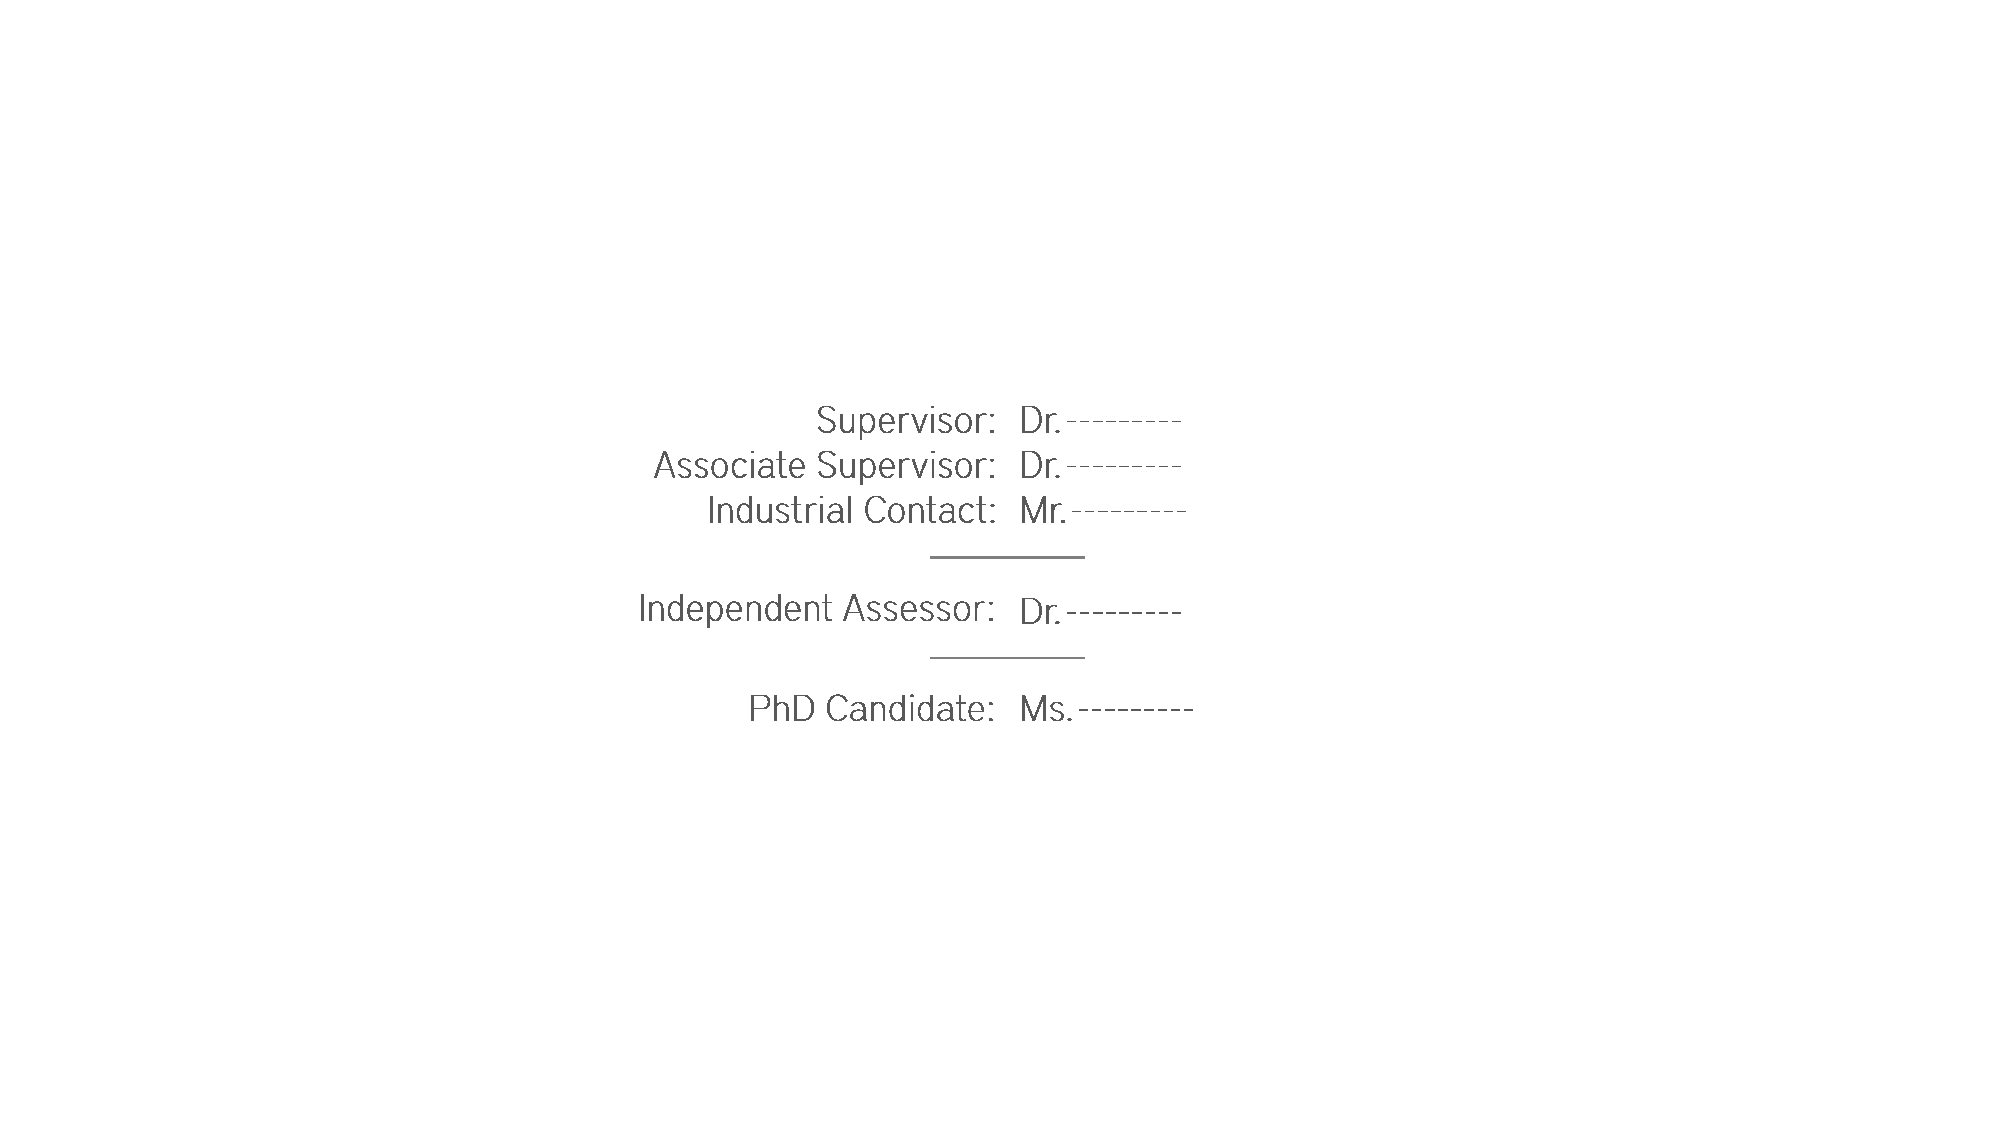
\includegraphics[scale=0.6]{Images/Supervisors}
	% \caption{Logo Caption Text}
	\label{fig:Supervisors}	% N.B. The label MUST be placed AFTER the caption for figures
\end{figure}

\end{center}

\thispagestyle{empty}	% Hides the page number from this page (note: this page is still counted). Also hides headers, footers, etc.

\newpage

%%%%%%%%%%%%%%%%%%%%%%%%%%%%%%%%%%%%%%%%%%%%%%%%%%%%%%%%%%%%%%%%%% Front Matter: Table of Contents Page %%%%%%%%%%%%%%%%%%%%%%%%%%%%%%%%%%%%%%%%%%%%%%%%%%%%%%%%%%%%%%%%%%

% \setcounter{page}{1}	% Starts the page numbering from this number

\renewcommand{\contentsname}{\hfill\bfseries\Large Contents\hfill}	% Places the 'Contents' title in the (horizontal) centre of the page

\tableofcontents\thispagestyle{fancy}	% Generates TOC at this location. \thispagestyle forces the TOC page to have the same header/footer as is defined globally / for the document

% \afterpage{\rfoot{\thepage}}	% Starts page numbering in this footer/header position on the following page (note: over-rides any previous definition for that footer/header)

\newpage

%%%%%%%%%%%%%%%%%%%%%%%%%%%%%%%%%%%%%%%%%%%%%%%%%%%%%%%%%%%%%%%%%% Front Matter: Nomenclature & Abbreviations Pages %%%%%%%%%%%%%%%%%%%%%%%%%%%%%%%%%%%%%%%%%%%%%%%%%%%%%%%%%%%%%%%%%%

\begin{center}
\section*{Nomenclature}	% Using an asterisk omits this section heading from the table of contents (it's neither counted as a section, nor displayed)
\end{center}
\renewcommand*{\arraystretch}{1.4}				% Values >1 increase the vertical spacing between the rows of the longtable containing the nomenclature
%\setlength{\extrarowheight}{.5em}
\begin{longtable}[l]{p{120pt} p{100pt} p{200pt}} \textbf{Symbol}	& \textbf{Units} & \textbf{Description} \\ 
	$\Delta V$ & $V$ & Change in voltage \\
	$k$ & $Varies$ & Coupling factor \\
	$E$ & $Pa$ & Young's modulus \\
	$x$ & $cm$ & Coordinate along the cell width \\
	$\kappa\SPSB{eff}{D}$ & $A/cm$ & Effective diffusional conductivity of the species \\
	$c\textsubscript{e}$ & $mol/cm\textsuperscript{3}$ & Volume-averaged concentration of lithium in the electrolyte phase \\
	$c\textsubscript{s}$ & $mol/cm\textsuperscript{3}$ & Volume-averaged concentration of lithium in the solid phase \\
	$i\textsuperscript{Li}$ & $A/cm\textsuperscript{3}$ & Reaction current resulting in production or consumption of lithium \\
\end{longtable}

\vspace{10mm}

\renewcommand*{\arraystretch}{1.0}	% Since the earlier, identical command also increases the row spacing for the glossary/list of abbreviations, we use the same command again here, but with a smaller value.
\printnoidxglossary[sort={word}, title={\centering Abbreviations}, toctitle={Abbreviations}]	% Place this line where the abbreviations should be printed. Title = title & toctitle = how it appears in TOC

\afterpage{\rfoot{\thepage}}	% Starts page numbering in this footer/header position on the following page (note: over-rides any previous definition for that footer/header)

\newpage

%%%%%%%%%%%%%%%%%%%%%%%%%%%%%%%%%%%%%%%%%%%%%%%%%%%%%%%%%%%%%%%%%% Document Body %%%%%%%%%%%%%%%%%%%%%%%%%%%%%%%%%%%%%%%%%%%%%%%%%%%%%%%%%%%%%%%%%%

\newpage

\setcounter{page}{1}	% Starts the page numbering from this number on this page

\section{\textbf{Project Definition}} \label{sec:project definition}

\subsection{Research question} \label{sec:research question}
The purpose of this project is to answer the following question:

\vspace{3mm}
\begin{quote} 
	\centering
	\textit{Research question goes here}
\end{quote}
% \vspace{3mm}

\subsection{Hypothesis} \label{sec:hypothesis}
\blindtext		% Example text only. Remove this line and replace it with your own content

\vspace{0.3cm}
\begin{quote} 
	\centering
	\textit{Hypothesis goes here}
\end{quote}
% \vspace{3mm}

\subsection{Scope} \label{sec:scope}
\blindtext		% Example text only. Remove this line and replace it with your own content

\subsection{Approach} \label{sec:approach}
\blindtext		% Example text only. Remove this line and replace it with your own content

\newpage

\section{\textbf{Topix X: An Introduction}} \label{sec:introduction}
\subsection{Context} \label{sec: context}
\blindtext		% Example text only. Remove this line and replace it with your own content 
\cite{Goodenough2010}	% Example citation

\begin{figure}[h]	% Sometimes, we use the begin / end{figure} setup so we can apply a position, e.g. 'b' or 'h' 
	\centering
	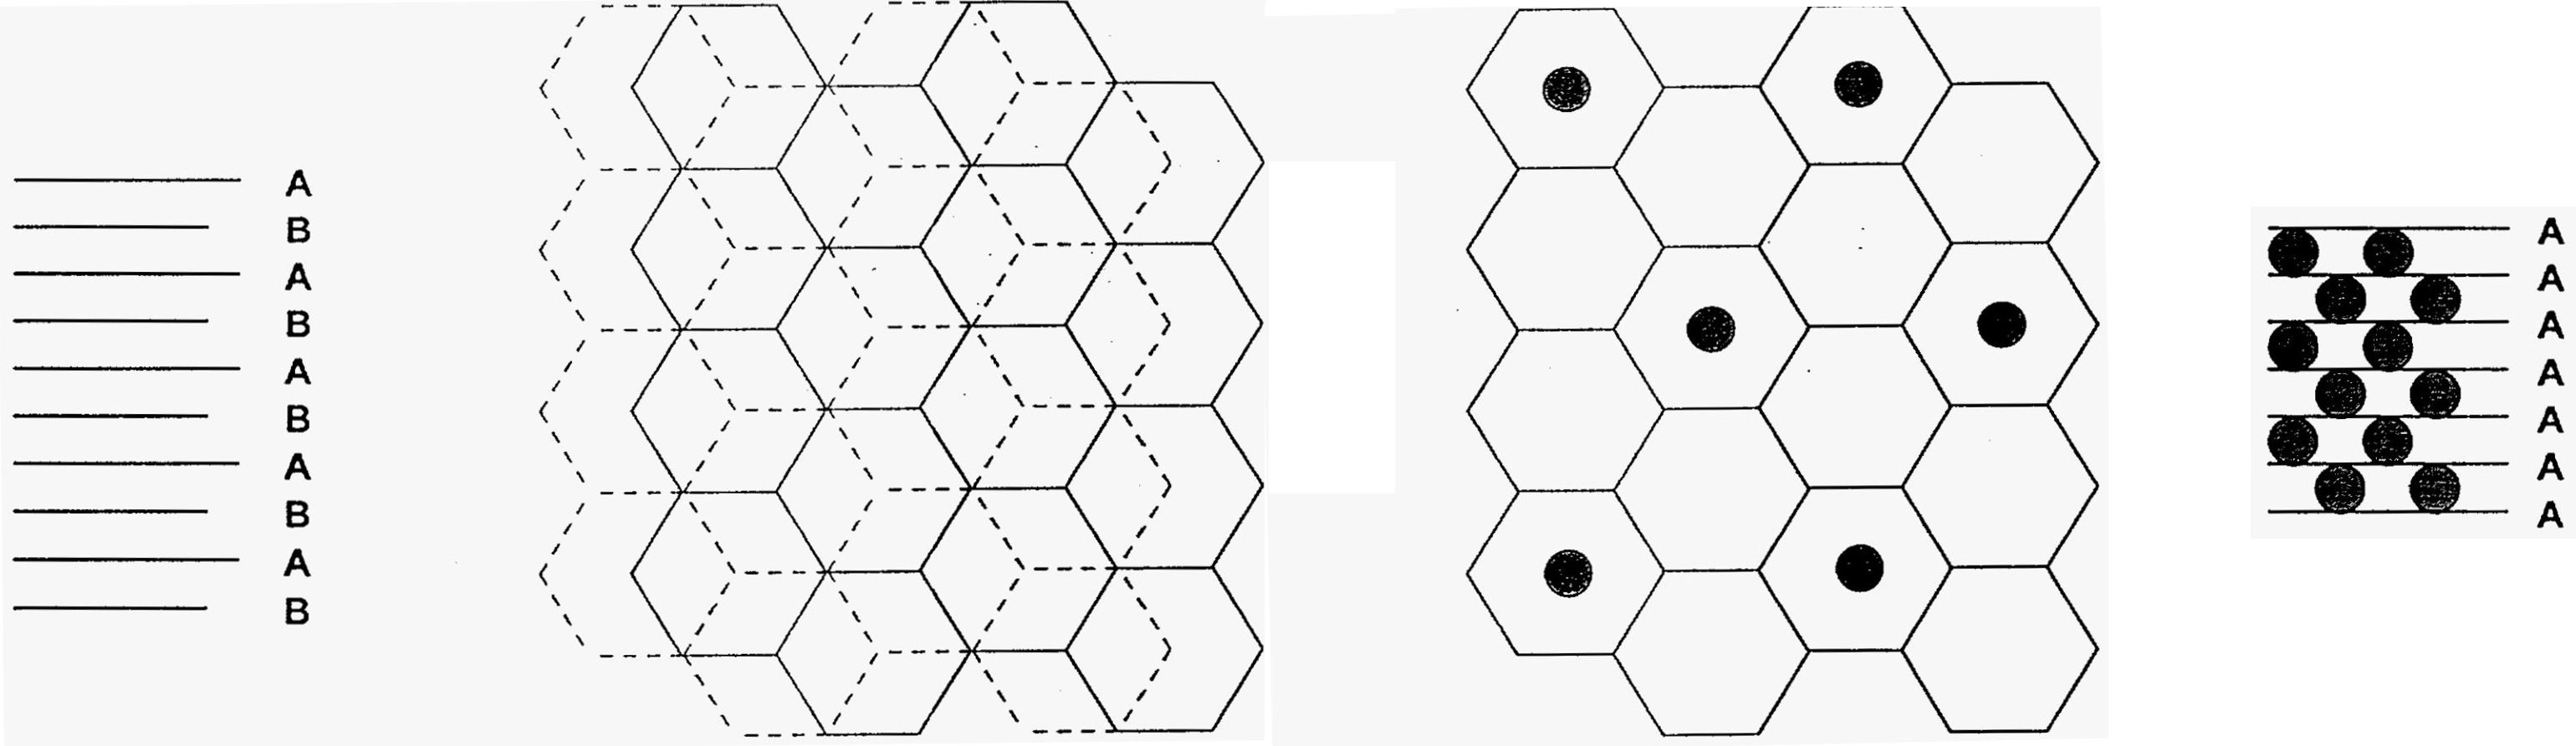
\includegraphics[scale=0.15]{Images/ABABAB_AAAA_Transition}
	\captionsetup{justification=centering}	% For caption text longer than 1 line, LaTeX doesn't center it. This line forces centering.
	\caption{Image caption text goes here \cite{1994Levy}.}
	\label{fig:graphite_structure}	% N.B. The label MUST be placed AFTER the caption for figures & caption MUST be included or label doens't work
\end{figure}

\blindtext		% Example text only. Remove this line and replace it with your own content 

\begin{figure}[h]	% Sometimes, we use the begin / end{figure} setup so we can apply a position, e.g. 'b' or 'h' 
	\centering
	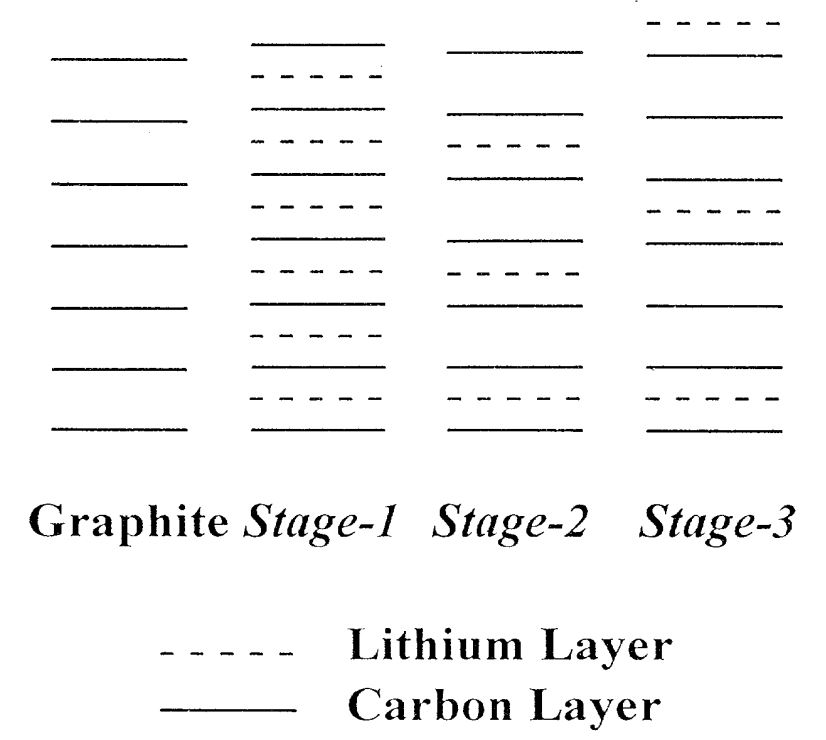
\includegraphics[scale=0.25]{Images/staging}
	\captionsetup{justification=centering}	% For caption text longer than 1 line, LaTeX doesn't center it. This line forces centering.
	\caption{Image caption text goes here \cite{Zheng1995} \cite{Yazami2006}.}
	\label{fig:staging}	% N.B. The label MUST be placed AFTER the caption for figures & caption MUST be included or label doens't work
\end{figure}

\blindtext		% Example text only. Remove this line and replace it with your own content 

\subsection{State of Knowledge} \label{sec:state of knowledge}
\blindtext \\	% Example text only. Remove this line and replace it with your own content

Here is an example of a citation \cite{Doyle1995a}. \\	% Example citation

Here is an example of acronym usage, where the acronym is called from the earlier-defined list: \gls{soc}. \\		% Example acronym usage

The Trajectory section, section \ref{sec:trajectory}, provides an example of how to perform linked section referencing, which is really useful! \\	% Example usage of section referencing. Note that using \linebreak instead of the double backslash to effet a linebreak can sometimes result in the awkward spacing of justified text.

\subsection{Doing Y in Topic X} \label{sec:doing Y}

\subsubsection{A sub-sub heading} \label{sec:short name for this section}
\blindtext		% Example text only. Remove this line and replace it with your own content

\begin{equation}\label{eq:species_cons_elec_phase}
	\frac{\delta\big(\epsilon\textsubscript{e}c\textsubscript{e}\big)}{\delta t} = \frac{\delta}{\delta x}\bigg(D\SPSB{eff}{e}\frac{\delta}{\delta x}c\textsubscript{e}\bigg)+\frac{1-t\SPSB{0}{+}}{F}i\textsuperscript{Li}
	\end{equation}

\blindtext		% Example text only. Remove this line and replace it with your own content

\subsubsection{Another sub-sub heading} \label{sec:short name for this section, 2}
\blindtext		% Example text only. Remove this line and replace it with your own content

\subsubsection{A sub-sub heading again} \label{sec:short name for this section, 3}
\blindtext		% Example text only. Remove this line and replace it with your own content

An example of section referencing is to call this section; \ref{sec:short name for this section, 2}. 

An example of citation is as follows... \cite{Goodenough2013a}

An example of in-line super and subscripts is as follows: 10\textsuperscript{-5} to 10\textsuperscript{-1}. Subscript here: 10\textsubscript{-1}

\subsection{Summary} \label{sec:literaturesummary}
An example of figure referencing is this line of text referring to Figure \ref{fig:theory_summary}.

\bigskip

\blindtext		% Example text only. Remove this line and replace it with your own content

\begin{figure}[h]	% Sometimes, we use the begin / end{figure} setup so we can apply a position, e.g. 'b' or 'h' 
	\centering
	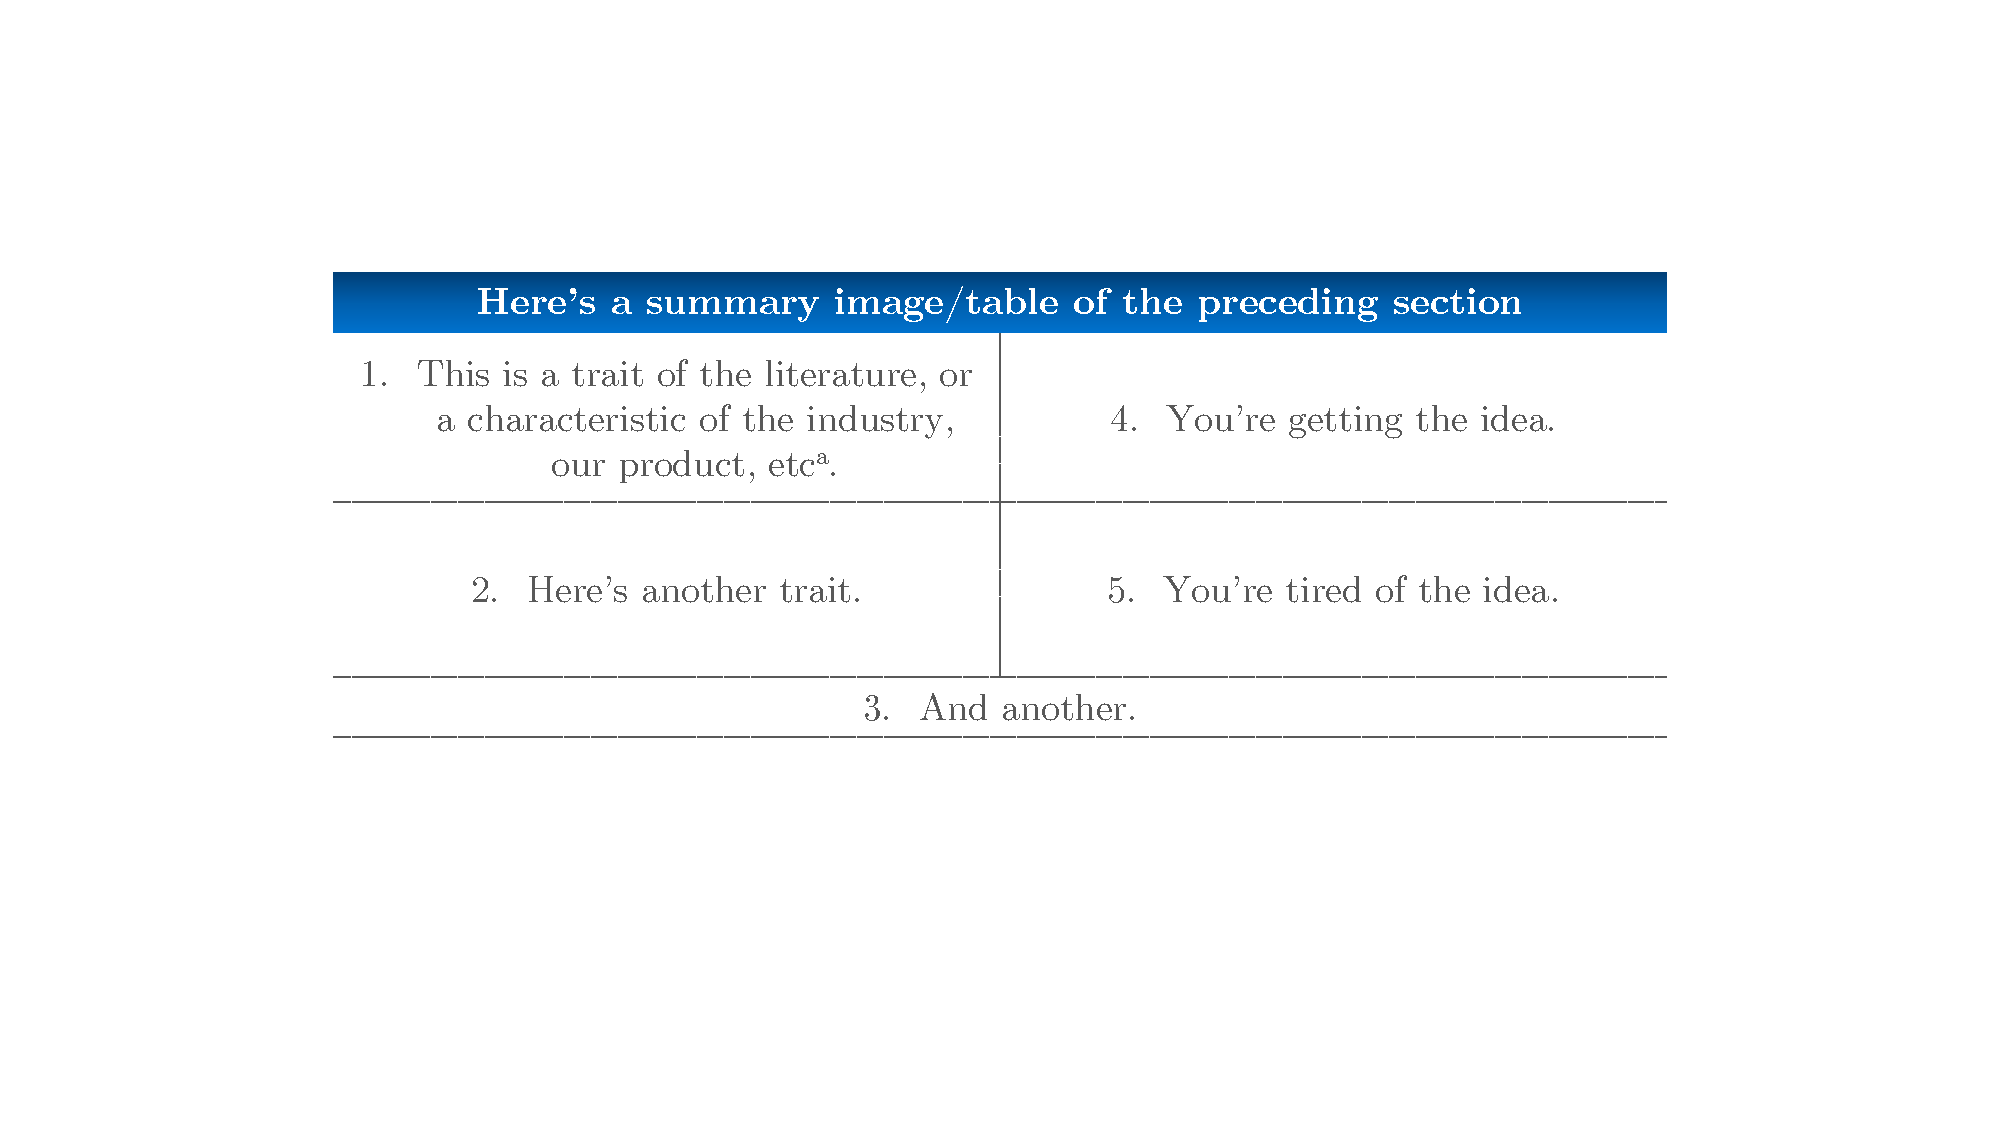
\includegraphics[scale=0.6]{Images/theory_summary}
	\captionsetup{justification=centering}	% For caption text longer than 1 line, LaTeX doesn't center it. This line forces centering.
	\caption{Here's a generic figure caption where a hypothetical superscript in the image coincides with that for at the following citation \textsuperscript{a}\cite{Goodenough2013a}}.
	\label{fig:theory_summary}	% N.B. The label MUST be placed AFTER the caption for figures & caption MUST be included or label doesn't work
\end{figure}

\newpage

\section{\textbf{Work to Date}} \label{sec:work to date}

\subsection{First Major Workpackage} \label{sec:First Major Body of Work}
\blindtext		% Example text only. Remove this line and replace it with your own content

\subsection{Second Major Workpackage} \label{sec:Second Major Body of Work}

\subsubsection{First Minor Workpackage} \label{sec:Name for 1st subsection of work package 2}
\blindtext \\		% Example text only. Remove this line and replace it with your own content

Here is a random example of some more figure referencing, where we refer to Figure number \ref{fig:Smith_Wang_Battery_Model}. \\	% Example of figure referencing

\blindtext		% Example text only. Remove this line and replace it with your own content

\begin{figure}[h] 
	\centering
	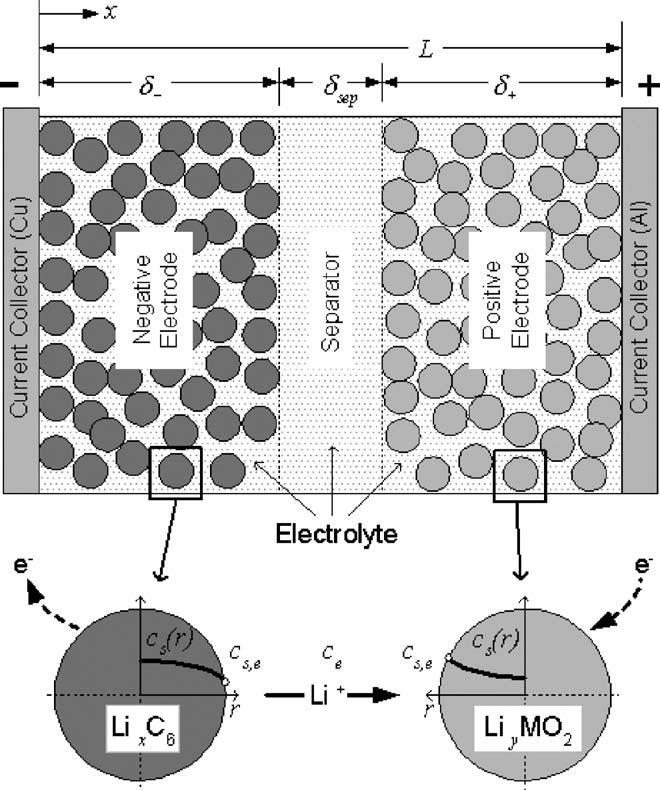
\includegraphics[scale=0.45]{Images/Smith_Wang_Battery_Model}
	\caption{Here's an image caption, and a reference \cite{Goodenough2013a}.}
	\label{fig:Smith_Wang_Battery_Model}
\end{figure}

% Example: Including mathematical equations in a LaTeX document

\begin{multicols}{2}
	\begin{center}
	
	\textit{Charge conservation, electrolyte phase}
	\begin{equation}\label{eq:charge_cons_elec_phase}
	\frac{\delta}{\delta x}\bigg(\kappa\textsuperscript{eff}\frac{\delta}{\delta x}\phi\textsubscript{e}\bigg)+\frac{\delta}{\delta x}\bigg(\kappa\SPSB{eff}{D}\frac{\delta}{\delta x}\ln c\textsubscript{e}\bigg)+i\textsuperscript{Li}=0
	\end{equation}
	
	\textit{Charge conservation, solid phase}
	\begin{equation}\label{eq:charge_cons_solid_phase}
	\frac{\delta}{\delta x}\bigg(\sigma\textsuperscript{eff}\frac{\delta}{\delta x}\phi\textsubscript{s}\bigg)-i\textsuperscript{Li}=0
	\end{equation}
	
	\textit{Lithium conservation, electrolyte phase}
	\begin{equation}\label{eq:species_cons_elec_phase}
	\frac{\delta\big(\epsilon\textsubscript{e}c\textsubscript{e}\big)}{\delta t} = \frac{\delta}{\delta x}\bigg(D\SPSB{eff}{e}\frac{\delta}{\delta x}c\textsubscript{e}\bigg)+\frac{1-t\SPSB{0}{+}}{F}i\textsuperscript{Li}
	\end{equation}
	
	\textit{Lithium conservation, solid phase}
	\begin{equation}\label{eq:species_cons_solid_phase}
	\frac{\delta c\textsubscript{s}}{\delta x} = \frac{D\textsubscript{s}}{r\textsuperscript{2}}\frac{\delta}{\delta r}\bigg(r\textsuperscript{2}\frac{\delta c\textsubscript{s}}{\delta r}\bigg)
	\end{equation}
	
	\end{center}
\end{multicols}

% Example (below): writing mathematical equations inline in LaTeX

We can write equations and symbols in formatted columns on in-line, like the following character in this line $c\textsubscript{e}$. We can also insert Greek symbols $\phi\textsubscript{e}$ and fractions, for example: $\frac{R\textsubscript{SEI}}{a\textsubscript{s}}i\textsuperscript{Li}$.

\begin{comment}
If you have a lot of text that add as a comment, you can place it within these commands instead of using a \% symbol for every line. If you have a LaTeX keyword, such as the \% symbol in LaTeX, you can prevent LaTeX from recognising it as a keyword  by placing a backslash immediately before it.
\end{comment}

\begin{equation}\label{eq:BV}
i\textsuperscript{Li} = a\textsubscript{s}i\textsubscript{0} \left[\exp[\frac{\alpha\textsubscript{a}F}{RT}(\eta\textsubscript{s}-\frac{R\textsubscript{SEI}}{a\textsubscript{s}}i\textsuperscript{Li})] - \exp[\frac{\alpha\textsubscript{c}F}{RT}(\eta\textsubscript{s}-\frac{R\textsubscript{SEI}}{a\textsubscript{s}}i\textsuperscript{Li})]\right]
\end{equation}

\bigskip

\subsubsection{Second Minor Workpackage} \label{sec:Name for 2nd subsection of work package 2}
\blindtext		% Example text only. Remove this line and replace it with your own content 

\subsection{Communication \& Learning}
\blindtext \\		% Example text only. Remove this line and replace it with your own content 

% Example of footnote usage in LaTeX:
If you'd like to include some text - or links - as footnotes, you can of course do that! Here's an example of two footnotes. \footnote{\url{https://someURL.com}}\footnote{\url{https://anotherURL.com}}

\clearpage % An alternative to \newpage, but with some differences..

\section{\textbf{Progression}}

\begin{figure}[h]	% Sometimes, we use the begin / end{figure} setup so we can apply a position, e.g. 'b' or 'h' 
	\centering
	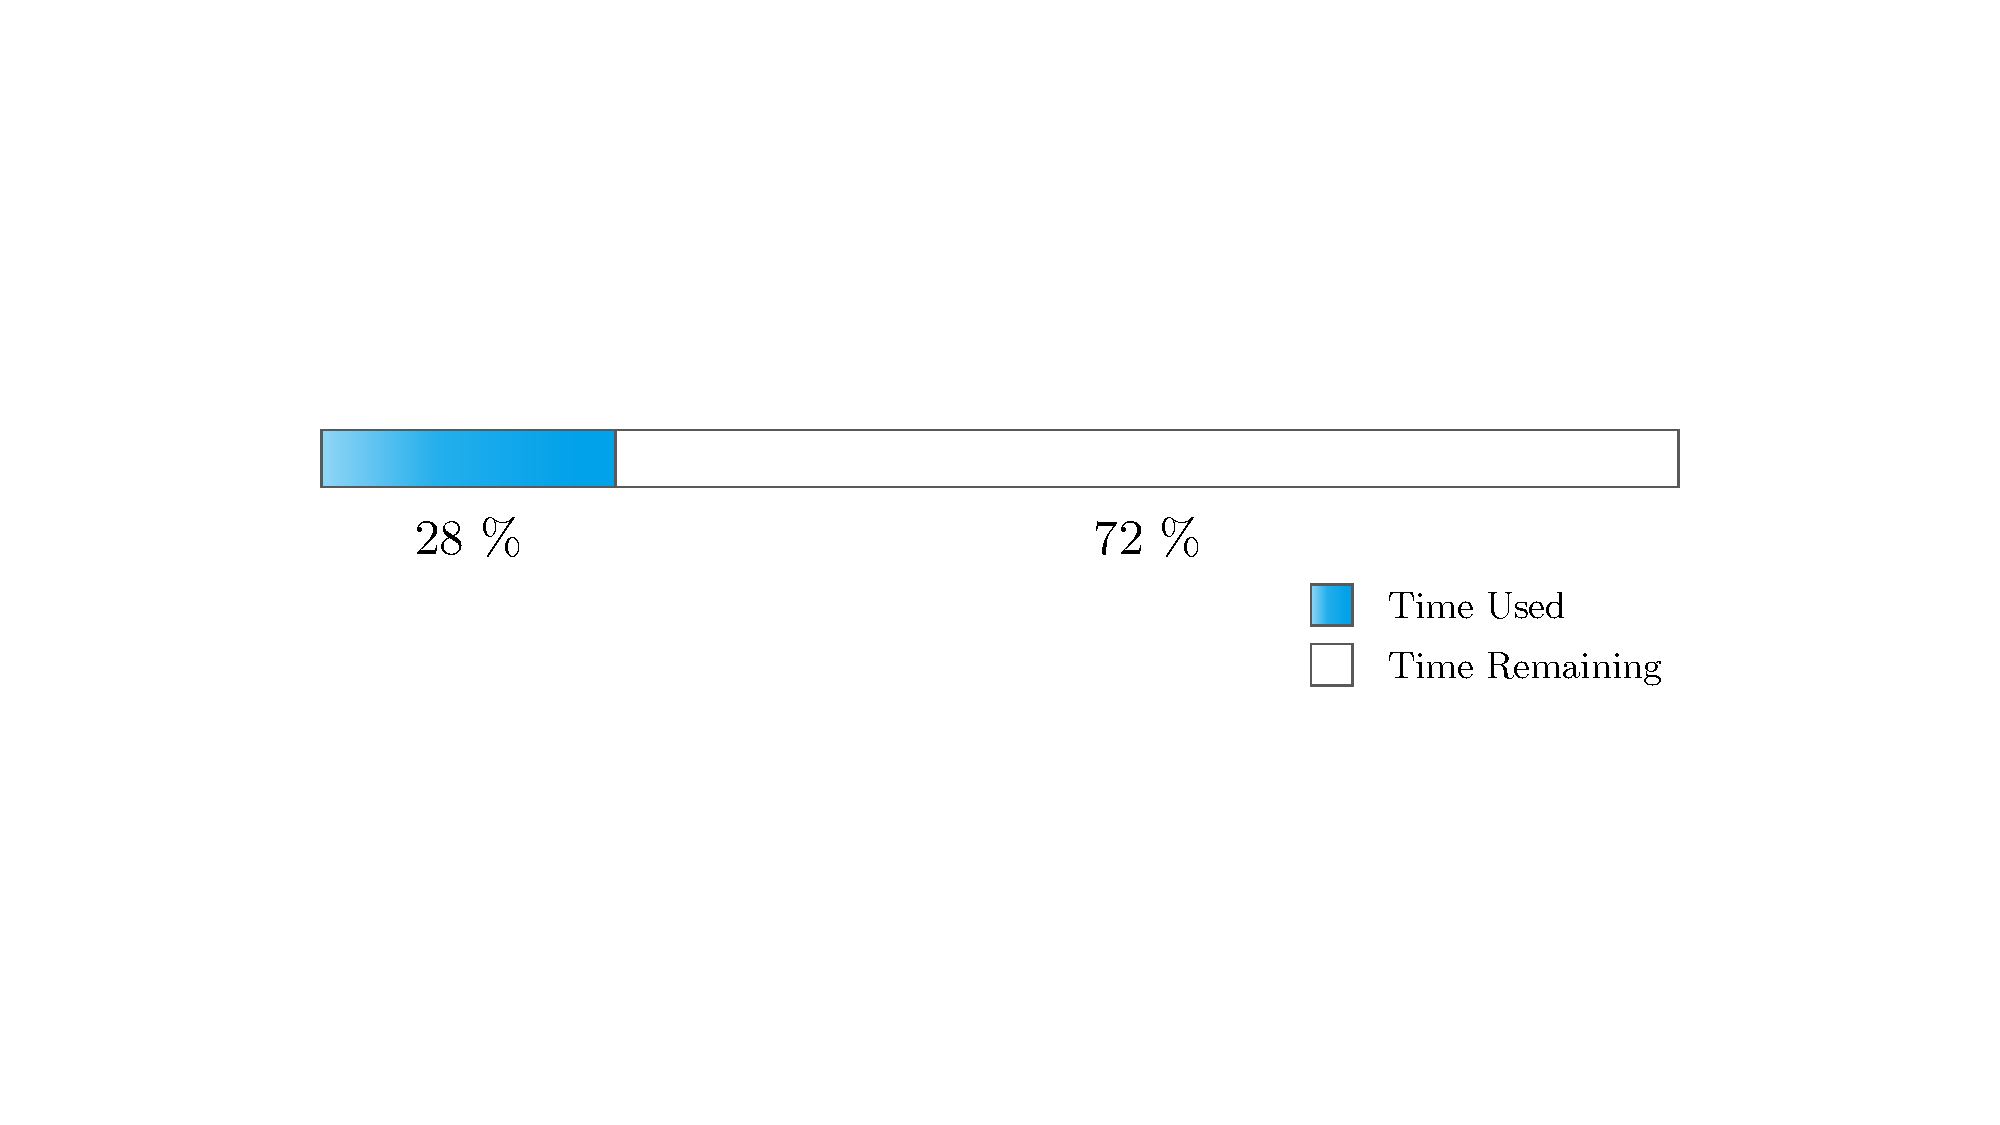
\includegraphics[scale=0.4]{Images/progress_bar}
	% \caption{Logo Caption Text}
	\label{fig:Progess_Bar}	% N.B. The label MUST be placed AFTER the caption for figures
\end{figure}

\blindtext		% Example text only. Remove this line and replace it with your own content 

\subsection{Trajectory} \label{sec:trajectory}
\blindtext		% Example text only. Remove this line and replace it with your own content 

\newpage

\newgeometry{top=1.2cm, bottom=1.2cm, outer=0cm, inner=1cm}

% Example of landscape page orientation in LaTeX

\begin{landscape}
\thispagestyle{empty}	% Removes the footer on this page for cleanliness, & because I can't find a good way to rotate it with the page content

\hfill	% Using both '\hfill' commands together here vertically centers the image on the page. 'hfill' rather than 'vfill' because commands still work as if portrait format

\begin{center}
	\begin{figure}[h] 
		\centering
		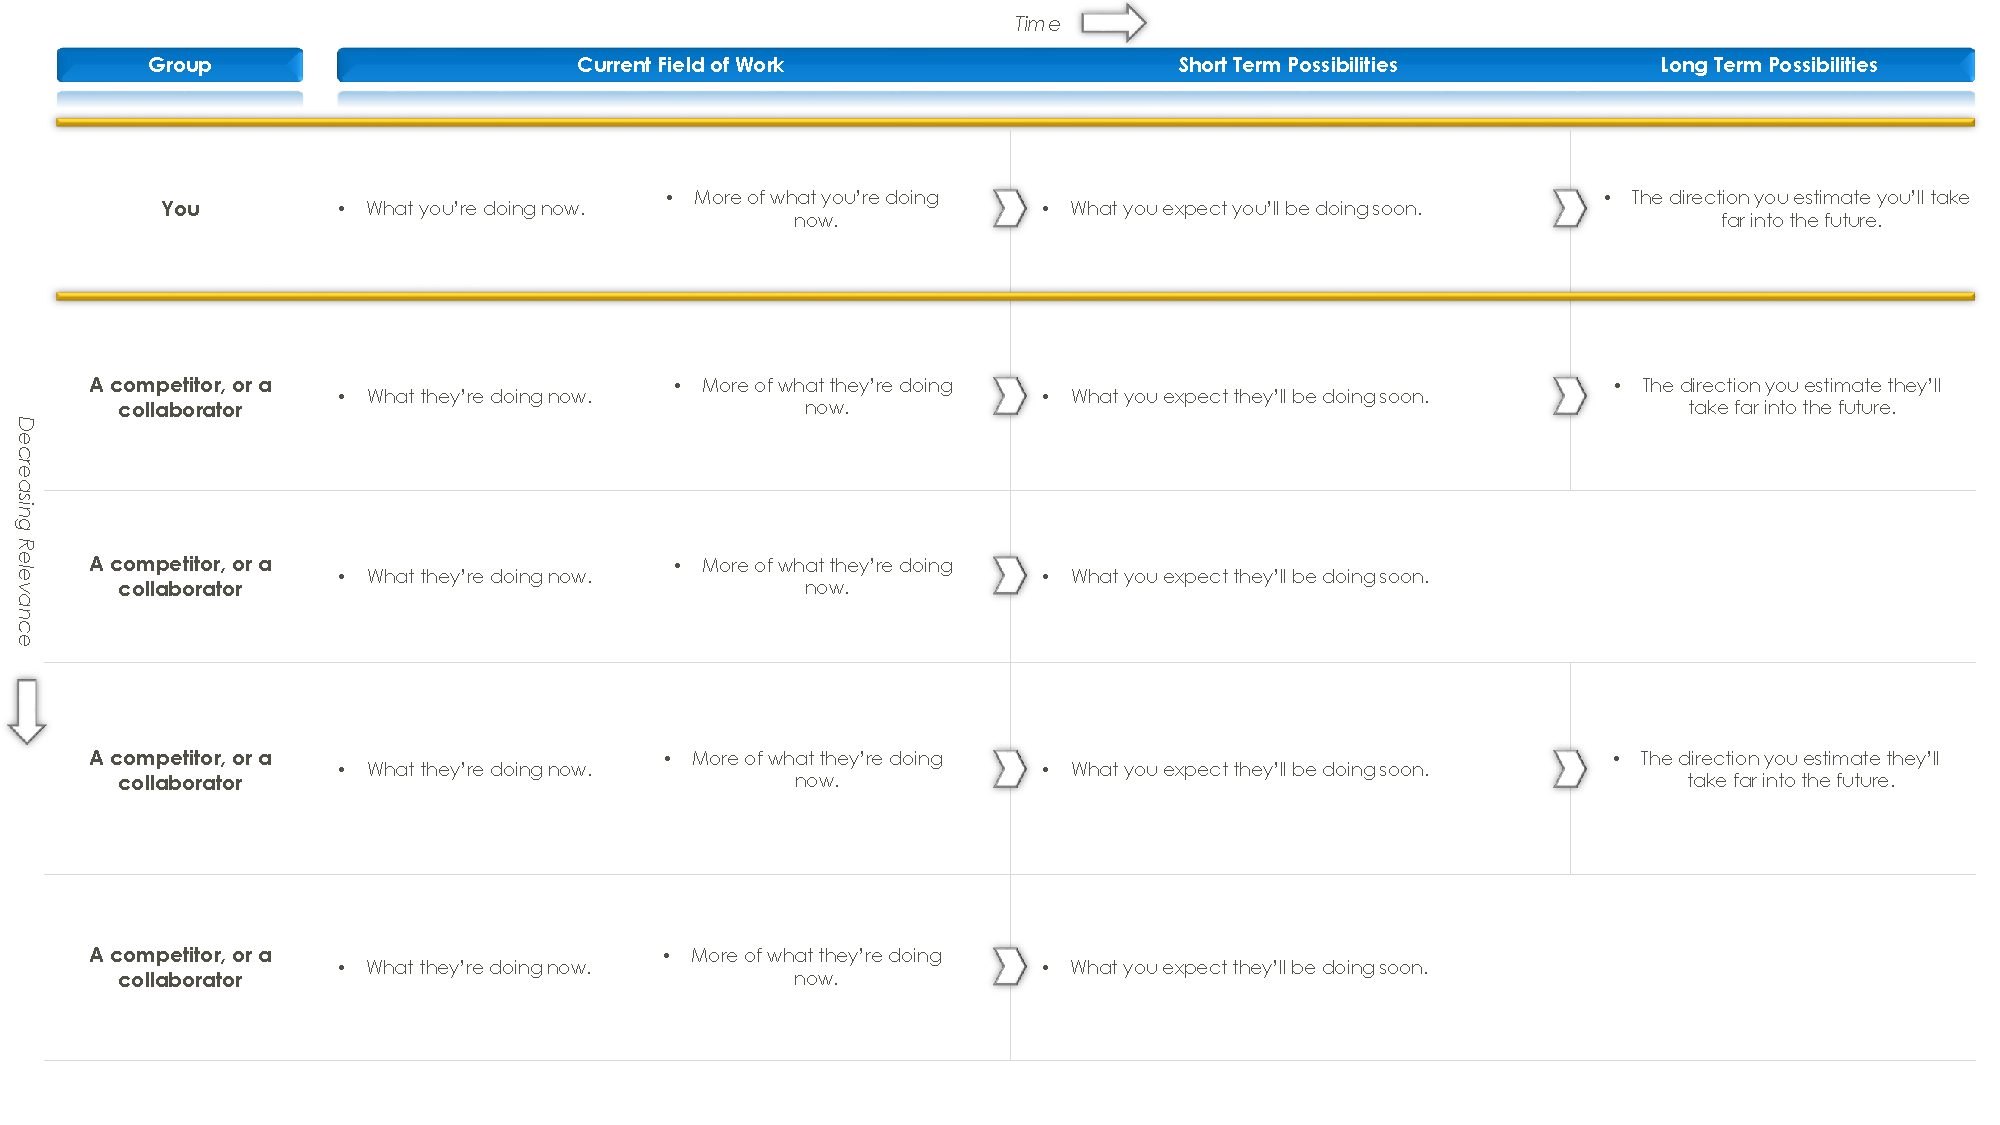
\includegraphics[scale=0.8]{Images/competitor_trajectories}
		\caption{Here's the caption text for the landscape-format image.}
		\label{fig:competitor_trajectories}	% N.B. The label MUST be placed AFTER the caption for figures & caption MUST be included or label doens't work
	\end{figure}
\end{center}

\hfill	% Using both '\hfill' commands together here vertically centers the image on the page. 'hfill' rather than 'vfill' because commands still work as if portrait format

\end{landscape}

\restoregeometry

\newpage

\subsection{Communication}
\blindtext		% Example text only. Remove this line and replace it with your own content

\section{\textbf{Conclusion}}
\blindtext		% Example text only. Remove this line and replace it with your own content

\subsection{Acknowledgements}
\blindtext		% Example text only. Remove this line and replace it with your own content

\vspace{10mm}

\includegraphics[scale=0.06]{Images/Signature}	% Can use 'width=\linewidth' or 'width=1.0\textwidth' instead of 'scale=0.45' either
\vspace{6mm}

\noindent	% Prevents indentation of the first line of the following paragraph
Author name \newline	% Creates a line break - equivalent to pressing the 'return' key. Also ensures the line is filled, so formatting remains in good condition
Address line one \newline
Address line two \newline
Address line three \newline
Phone: +00 (0)0000 000 000 \newline
E-mail: ------------@domain.com \newline

\vspace{20mm}

\clearpage	% Adds a page break (N.B. Difference to \newpage is that \clearpage truly starts a new page, whereas \newpage just ends the current column & doesn't work in 2-column mode)

%%%%%%%%%%%%%%%%%%%%%%%%%%%%%%%%%%%%%%%%%%%%%%%%%%%%%%%%%%%%%%%%%% End of Document Body %%%%%%%%%%%%%%%%%%%%%%%%%%%%%%%%%%%%%%%%%%%%%%%%%%%%%%%%%%%%%%%%%%

%% Single column bibliography/references layout: use this code segment %%
%\bibliography{BibTeX_Libraries/Report Sample}		% Prints the bibliography at this location. Don't write the ".bib" file extension. Place the .bib file in the same location as the .tex and no absolute path is needed
%% End %%

%% Two-column bibliography/references layout: use this code segment %%
\section{References}	% Manually sets the section heading 'References' so that it is OUTSIDE of the 2-column environment & includes it in the table of contents, since no asterisk is used
\addtocontents{toc}{\cftpagenumbersoff{section}}	% Supresses the page number that would otherwise show because of the '\renewcommand' function in the code below
\begin{multicols}{2}	% Begins the 2-column reference environment using the 'multicol' package
	\small	% Adjusts the font size for text in the columns. 'Actual size is not absolute but relative to the font size declared in the \documentclass statement'.
	\renewcommand{\refname}{ \vspace{-\baselineskip}\vspace{-1.1mm} }	% Shifts the starting point of the 2nd column down so it begins in-line with the 1st column.
	\bibliographystyle{unsrt}		% {stylename} argument can take; abbrv / acm / alpha / apalike / ieeetr / plain / siam / unsrt (unsrt = entries appear in order of citation & are labeled numerically)
	\renewcommand{\section}[2]{}	% Hides the section number that would appear without this line. Doesn't hide page number in the table of contents though. Need \cftpagenumbersoff (used above) for this
	\bibliography{BibTeX_Libraries/Sample_refs}	% Prints the bibliography at this location. Don't write the ".bib" file extension. Place the .bib file in the same location as the .tex and no absolute path is needed
\end{multicols}
\addtocontents{toc}{\cftpagenumberson{section}} % to restore the showing of page numbers
%% End %%

\end{document}

%%%%%%%%%%%%%%%%%%%%%%%%%%%%%%%%%%%%%%%%%%%%%%%%%%%%%%%%%%%%%%%%%% End %%%%%%%%%%%%%%%%%%%%%%%%%%%%%%%%%%%%%%%%%%%%%%%%%%%%%%%%%%%%%%%%%%
